\documentclass[../DCM2_Verslag.tex]{subfiles}
\begin{document}

Dit hoofdstuk gaat kort in op achtergrond informatie die benodigd is om bepaalde delen van het onderzoek te kunnen begrijpen.
\\
De eerste sectie van dit hoofdstuk geeft de benodigde achtergrond informatie over embedded systemen.
\\
De tweede sectie gaat over tcp/ip stacks
\\
De derde sectie gaat over sockets

\section{Embedded systemen}
Embedded systemen is een woord van de laatste jaren, maar embedded systemen bestaan al veel langer. Het enige wat nodig is, is een blik werpen op de apparaten om je heen: Telefoons, Modems, Televisies en koffie apparaten om een paar voorbeelden te noemen. 
\\
Deze sectie geeft een korte introductie in embedded systemen.

\subsection{Het verschil tussen een computer en embedded systeem}
Een embedded systeem wordt vaak beschreven als een systeem die een bepaald aantal vaste taken moet uitvoeren met beperkte ingebouwde functionaliteit. Dit zijn bijna altijd onzichtbare mini computers (microcomputers) die ingebouwd zitten in apparaten. Maar het kunnen ook chips met programmeerbare hardware zijn (FPGA's of CPLD's). 
\\
Het grote verschil tussen een computer en een embedded systeem is het doeleind. Embedded systemen zijn ontworpen voor een specifieke taak en zijn vaak alleen goed in deze taak. Normale computers daarentegen zijn gemaakt om verschillende uiteenlopende taken goed uittevoeren. Doordat een embedded systeem vaak maar een taak heeft zijn embedded systemen vaak uitgerust met veel minder geheugen en (algemene) computerkracht dan een normaal computersysteem.

\subsection{Het ontwerp van embedded systemen}
Zoals hierboven toegelicht zijn embedded systemen vaak ontworpen voor een specifiek aantal vaste taken. Zaken waar vaak rekening mee gehouden moet worden bij het ontwerpen van een embedded systeem zijn onder andere: reactie tijd nauwkeurigheid, formaat, energie verbruik en kosten. 
\\\\
Reactie tijd is een belangrijk begrip in het embedded domein. Of het hier gaat of het een taak is die op een bepaalde tijd wordt uitgevoerd (zoals een alarmklok) of de tijd tussen twee taken (zoals bij het geven van medicatie via infuuspompen) het kan een heel grote rol spelen in het ontwerp van het embedded systeem. Het moeilijkst is dan ook om deze tijden te bepalen, en vervolgens te bepalen of het strakke deadlines zijn die niet overschreden mogen worden. Zodat vervolgens in het ontwerp zoveel mogelijk gedaan kan worden om deze tijden te waarborgen. 
\\\\
Formaat van het systeem is ook een belangrijke weging. Veel embedded systemen die in dezer dagen verkocht worden, worden vaak verkocht omdat ze kleiner zijn dan hun voorganger(s). Neem als voorbeeld de smartphone, deze is door de jaren heen steeds kleiner en populairder geworden.
\\\\
Een andere belangrijke weging in het ontwerp van een embedded systeem is energieverbruik. 
Verder gaande op wat hier boven staat, worden veel embedded systemen kleiner. De accu's of batterijen die deze systemen voeden worden niet kleiner. Met als gevolg dat embedded systemen zuiniger moeten worden om op een kleinere batterij of accu te kunnen werken.
\\\\
Ten slotte het laatste punt kosten. Ondanks alle punten hierboven, als het systeem heel veel kost zal het niet verkopen. Meestte eindgebruikers leveren graag een beetje performance of batterijduur in om een goedkoper product te hebben. Bij de ontwerpfase is het zeer belangrijk om het kostenplaatje in de gaten te houden bij een toevoeging aan of modificatie van het ontwerp.


\section{TCP/IP stacks}
Het tcp/ip model is een van de fundamentele bouwstenen van het huidige internet infrastructuur. Het model bestaat uit vier lagen, zie figuur 1.\\
\begin{figure}[h]
\centering
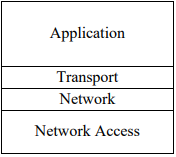
\includegraphics[scale=2]{tcp_ip_model}
\caption{TCP/IP model}
\end{figure}
De functies van de tcp/ip lagen zijn:
- De netwerk laag: Deze laag komt overeen met de fysieke en data link laag in het osi model. Deze laag is verantwoordelijk voor de data transmissie over een netwerk, het definieert hoe twee apparaten fysiek met elkaar moeten communiceren.
\\
- De internet laag: Deze laag stuurt data van het bron apparaat naar apparaten in het pad tussen het bron en doel apparaat. Het IP protocol neemt het grootste deel van deze taak op zich.
\\
- De transport laag: Deze laag zorgt ervoort dat de data bij de juiste applicatie geleverd wordt. Er zijn twee protocollen die deze taak kunnen vervullen: TCP en UDP. TCP is verantwoordelijk voor het bieden van een betrouwbare, verliesloos connetie georienteerde verbinding. UDP daarentegen is verantwoordelijk voor onbetrouwbare connectieloze verbinding tussen twee hosts.
\\
- De applicatie laag: Deze laag verzorgt de communicatie tussen de transport laag en de software applicaties. Dit doet de laag met protocollen zoals: HTTP, HTTPS, FTP, SMTP, enz.
\\

\subsection{Implementatie van TCP/IP stacks}
Er zijn twee soorten TCP/IP stack implementaties; Een is de TCP/IP stack afgeleid van de BSD implementatie en de andere is een door de embedded systeem fabrikant zelf geimplementeerde versie.\\
BSD is een besturingssysteem afgeleid van het UNIX besturingssysteem. BSD wordt nog weleens gebruikt op workstations en servers. Maar het was vroeger prominent aanwezig, doordat het zo prominent aanwezig was, hebben veel besturingssystemen zoals Linux met een kleine aanpassing de BSD implementatie voor de TCP/IP stack geadopteerd.
\\
Embedded systemen kunnen vaak door hardware limitaties niet de volledige BSD TCP/IP stack gebruiken. Om het toch werkend te krijgen op de hardware wordt de TCP/IP stack door de fabrikant van het embedded systeem versimpeld. Ondanks dat de TCP/IP stack versimpeld is, probeert de fabrikant toch de TCP/IP stack zoveel mogelijk compatibel te maken met de volledige TCP/IP stack die te vinden is in normale besturingssystemen. 
\\
De manier waarop de TCP/IP stack versimpeld kan worden, is het optimaliseren naar de hardware en software van het embedded systeem.
\\\\
Neem als voorbeeld een webserver:
\\\\
Een webserver is gebouwd met een simpele webinterface met alleen een paar knoppen erop. Deze implementatie heeft alleen de protcollen: HTTP, TCP, RARP, ARP en ICMP nodig. Protocollen zoals FTP en SNMP zijn in deze implementatie niet nodig. Deze protocollen kunnen dan ook verwijderd worden uit de broncode om betere prestaties en een kleinere geheugen footprint te creeren.


\section{Sockets}
Sockets zijn vaak onderdeel van een TCP/IP stack API die het mogelijk maakt om met behulp van de TCP/IP stack een directe TCP of UDP verbinding te maken met een andere host. Ook socket API's zijn vaak afgeleid van de BSD implementatie, maar het kan ook een custom implementatie zijn gemaakt door de fabrikant van het embedded systeem. 
\\\\
Een socket bestaat uit een IP-adres en een poort nummer. Sockets hebben geen bron adres nodig, standaard zijn sockets geconfigureerd om alleen te sturen en niet te ontvangen. Om toch data te ontvangen, kan een socket zichzelf vastmaken(binden) aan een lokaal adres.
\end{document}
